 \section{Adapted SEP ODP}\begin{description}
\item [ALSO KNOWN AS:] Transitive propagator.

\item [CLASSIFICATION:] Domain Modelling.

\item [MOTIVATION:] In the biomedical domain the propagation of properties along the partonomy relation is very important. For example, there are cases where the fault of the part should be assumed to be a fault of the whole (an appendix perforation is an intestine perforation) and other cases where it should not be considered like that (appendicitis is not enteritis). The problem of propagating properties along partonomy relates directly to the problem of (for example) overloading PartOf in the Gene Ontology: for example Location, a property that should propagate along (or not) with PartOf , is always implicitly present anywhere there is a PartOf relation. For example Polarisome is PartOf  CellCortex and PartOf SiteOfPolarizedGrowth, inheriting both locations, creating a conflict: polarisome is not located in the whole of the cell cortex, is only located in the cell cortex in the site of polarised growth.

\item [AIM:] To model selective transitive propagation.

\item [STRUCTURE:] See Figure \ref{odp:AdaptedSEP_abstract}.
\begin{figure}[]\centering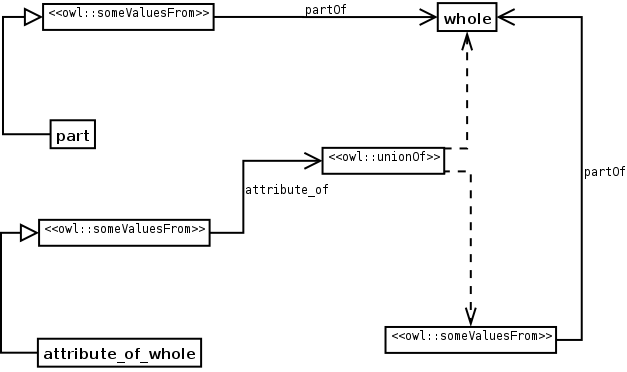
\includegraphics[width=\textwidth]{Catalogue/AdaptedSEP_abstract}\caption{\label{odp:AdaptedSEP_abstract} Abstract structure of the Adapted SEP ODP.}\end{figure}

\item [SAMPLE:] See Figure \ref{odp:AdaptedSEP_instance}.
\begin{figure}[]\centering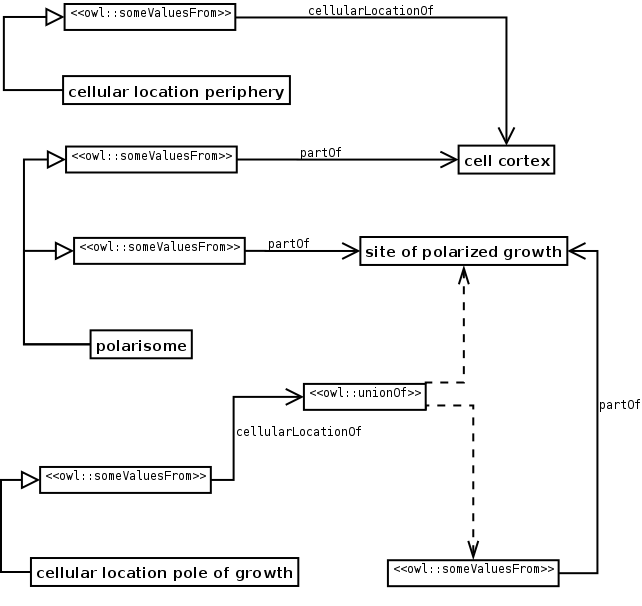
\includegraphics[width=\textwidth]{Catalogue/AdaptedSEP_instance}\caption{\label{odp:AdaptedSEP_instance} Sample structure of the Adapted SEP ODP.}\end{figure}

\item [ELEMENTS:] The elements of the partonomy hierarchy are maintained and in this case two new elements are added to represent concrete locations in the cell (CellularLocationPole and CellularLocationPeriphery). The PartOf relationship is maintained (defined as transitive) and in this case a new object property is added to link locations with cellular components, CellularLocationOf.

\item [IMPLEMENTATION:] The most important step is to define the class CellularLocationPoleOfGrowth as the location of SiteOfPolarizedGrowth or any of its parts, so the location is propagated to the parts (but it is not propagated in the case of CellCortex).

\item [RESULT:] The location property CellularLocationOf is propagated along PartOf in a selective way, allowing for a precise and unambiguous definition of the polarisome location. To check the result two classes can be created: PolarisomeLocation [partial CellularLocationOf some Polarisome] and SiteOfPolarisedGrowthLocation [complete cellularLocationOf some (SiteOfPolarisedGrowth and PartOf some SiteOfPolarisedGrowth)]. After reasoning PolarisomeLocation should be a subclass of SiteOfPolarisedGrowthLocation.

\item [ADDITIONAL INFORMATION:] There have been different proposals in the literature for modelling transitive propagation in the biomedical domain. The approach chosen for this ODP relies on the possibility of creating transitive object properties given by OWL DL. Another approach is the one described by Stefan Shultz and Udo Hahn (see references), which relies in simulating the transitivity by creating SEP triples (Structure - Entity - Part) for each class of the partonomy hierarchy, allowing for selective inheritance of properties.

\item [REFERENCES: ] ~\begin{itemize}
\item Alan L Rector and Sebastian Brandt. Why do it the hard way? The Case for an Expressive Description Logic for SNOMED.  JAMIA (28 August 2008).
\item \url{http://www.w3.org/2001/sw/BestPractices/OEP/SimplePartWhole/}
\item Julian Seidenberg, Alan Rector. "Representing transitive propagation in OWL". ER2006.
\item Stefan Shultz and Udo Hahn. Part-whole representation and reasoning in formal biomedical ontologies. Artificial Intelligence in Medicine, 34: 179-200, 2005.\end{itemize}
\item [URL: ] \url{http://www.gong.manchester.ac.uk/odp/owl/Domain_Modelling_ODP/Adapted_SEP.owl} \end{description}